\documentclass{ieeeaccess}
\usepackage{cite}
\usepackage{amsmath,amssymb,amsfonts}
\usepackage{algorithmic}
\usepackage{graphicx}
\usepackage{textcomp}

\usepackage{bm}
\makeatletter
\AtBeginDocument{\DeclareMathVersion{bold}
\SetSymbolFont{operators}{bold}{T1}{times}{b}{n}
\SetSymbolFont{NewLetters}{bold}{T1}{times}{b}{it}
\SetMathAlphabet{\mathrm}{bold}{T1}{times}{b}{n}
\SetMathAlphabet{\mathit}{bold}{T1}{times}{b}{it}
\SetMathAlphabet{\mathbf}{bold}{T1}{times}{b}{n}
\SetMathAlphabet{\mathtt}{bold}{OT1}{pcr}{b}{n}
\SetSymbolFont{symbols}{bold}{OMS}{cmsy}{b}{n}
\renewcommand\boldmath{\@nomath\boldmath\mathversion{bold}}}
\makeatother

\def\BibTeX{{\rm B\kern-.05em{\sc i\kern-.025em b}\kern-.08em
    T\kern-.1667em\lower.7ex\hbox{E}\kern-.125emX}}

\begin{document}
\history{Date of publication xxxx 00, 0000, date of current version xxxx 00, 0000.}
\doi{10.1109/ACCESS.2024.0429000}

\title{Design and Formative Evaluation of a Real-Time Liver Palpation Simulation System Based on Group-Based Corotational FEM and a 1-DOF Haptic Interface}
\author{\uppercase{Yunxiu Xu}\authorrefmark{1}, \uppercase{Shugo Hasegawa}\authorrefmark{1}}
\address[1]{School of Fundamental Science and Engineering, Waseda University, Tokyo, Japan}
\corresp{Corresponding author: Yunxiu Xu (e-mail: placeholder@waseda.jp).}

\begin{abstract}
This paper presents a real-time system prototype for liver lesion palpation training that integrates a previously published Group-Based Corotational Finite Element Method (GB-cFEM) solver, bimanual Ultraleap Stereo IR-170 tracking, and a 1-DOF haptic interface. Hidden lesions are represented through local stiffness enhancement, and the contact-normal reaction force is mapped to single-axis haptic output to amplify stiffness contrast between healthy tissue and pathological regions. On the basis of prior evidence that the simulation core supports real-time large deformation and volume preservation, this study focuses on system-level formative evaluation. A preliminary clinical localization observation suggests that even with a lightweight 1-DOF haptic channel, targeted force feedback may alter the operator's lesion-search strategy and support perception of local resistance differences. Because the clinical session used a single participant and non-counterbalanced lesion conditions, the evidence is descriptive rather than causal. Overall, the study indicates that a physics-based low-complexity haptic design has the potential to provide effective interaction gains for soft-tissue palpation training, while offering a feasible integration and evaluation framework for low-cost, portable medical training platforms.
\end{abstract}

\begin{keywords}
Liver palpation, real-time simulation, corotational finite element method, XPBD, Stereo IR-170, 1-DOF haptic interface, medical training.
\end{keywords}

\titlepgskip=-21pt
\maketitle

\section{Introduction}
In the development of modern minimally invasive medicine and surgical planning, the simulation of abdominal organ palpation has become an important topic at the intersection of medical engineering and computational mechanics. Palpation of highly vascularized soft tissues such as the liver is not only a key means of assessing lesion distribution, boundary shape, and local stiffness changes, but also an essential step through which surgeons accumulate experience and develop muscle memory. Reproducing this process in a virtual or augmented environment is difficult because the system must simultaneously handle large soft-tissue deformation, real-time visual updates, and haptic interaction.

From the computational perspective, soft tissues under pressing and traction exhibit nonlinear, large-deformation, and near-incompressible behavior. Traditional nonlinear finite element methods can provide strong physical consistency, but at a high computational cost. Fast graphics-oriented approaches such as XPBD provide strong real-time performance, yet often lack clearly interpretable material parameters. From the interaction perspective, multi-degree-of-freedom force-feedback devices can provide richer kinesthetic information, but they are often bulky, have high inertia, limited workspace, and high cost, which makes them less suitable for portable and low-threshold training platforms.

Existing studies often emphasize solver accuracy, interaction convenience, or hardware realism separately, but fewer works address all of the following within one system: physically meaningful large soft-tissue deformation, real-time interaction on consumer-grade computing platforms, bimanual exploratory input, and an effective low-complexity haptic interface for lesion localization. This gap is particularly evident in liver palpation training, where lesion detection depends strongly on local stiffness contrast rather than visual surface deformation alone.

To address this problem, this paper proposes a real-time liver palpation system based on Group-Based Corotational FEM (GB-cFEM), Ultraleap Stereo IR-170 bimanual input, and a 1-DOF haptic interface. Hidden lesions are simulated by local stiffness enhancement, and the contact-normal reaction force is mapped to single-axis haptic output to emphasize stiffness differences between normal and pathological regions. Unlike prior work centered mainly on algorithmic derivation, this paper focuses on how an already validated physics core can be integrated into a complete interactive system and whether it can deliver practical task-level benefits for lesion localization.

It should be noted that the GB-cFEM simulation core and its systematic algorithmic validation were previously published in \cite{ref6}. Accordingly, the aim of this paper is not to repeat a universal proof of solver performance, but to present its integration into a liver palpation system and to investigate its application potential at the task level. The main contributions of this paper are as follows:
\begin{enumerate}
\item We build a complete interactive system for liver lesion palpation training by integrating a published GB-cFEM core, bimanual visual tracking, and 1-DOF haptic output.
\item We propose and implement a low-dimensional haptic mapping strategy and a hidden-lesion configuration workflow tailored to lesion-search tasks.
\item Through expert formative evaluation and task-level observation, we provide an initial analysis of the interaction value of haptic feedback and its potential effect on lesion-localization strategy.
\end{enumerate}

\section{Related Work}
Interactive simulation systems for surgical training and palpation skill acquisition require engineering tradeoffs among visual rendering rate, haptic update rate, and physical modeling complexity. Reviews on medical simulation note that the value of virtual reality and haptic systems depends not only on tissue mechanics and real-time performance, but also on task definition, evaluation protocol, and educational evidence \cite{ref1,ref2,ref3,ref4}. For the liver palpation task studied here, the most relevant prior work falls into three lines: real-time soft-tissue modeling, liver-related training systems, and low-dimensional haptic rendering.

\subsection{Real-time soft-tissue modeling for surgical simulation}
Continuum-based FEM remains a standard choice in surgical simulation because it represents material parameters, boundary conditions, and volumetric meshes naturally, but real-time performance becomes challenging under large deformation, near incompressibility, contact, and cutting. Co-rotational formulations alleviate part of this burden by separating large rigid rotation from strain evaluation, and have been extended to surgical settings such as needle insertion and cutting \cite{ref5}. More recently, group-based and domain-decomposition strategies have pushed this line further on multicore CPUs. In particular, GB-cFEM combines grouped local solves, offline precomputation, and iterative inter-group coupling, while supporting anisotropic and near-incompressible cases at interactive rates \cite{ref6}. This route is directly relevant to our system because it preserves material meaning better than purely geometric methods while remaining practical for real-time liver deformation.

In parallel, optimization-based approaches such as Projective Dynamics and its hyperelastic extensions offer an alternative balance between stability and speed \cite{ref7,ref8}, and constraint-energy formulations have also been used to build interactive soft-tissue models with stronger physical consistency \cite{ref17}. By contrast, PBD and XPBD are widely adopted as efficient engineering baselines because of their robustness and ease of implementation, although they generally prioritize controllability over strict mechanical fidelity \cite{ref9,ref10,ref11}. For lesion palpation tasks that rely on stiffness contrast, anisotropy, and near-incompressible behavior, continuum-based FEM remains the more suitable main model.

\subsection{Liver-related simulation systems and training tasks}
Research on liver and abdominal-organ simulation covers both deformation-and-cutting workflows and palpation-centered diagnostic tasks. For example, prior work has reported haptic liver-transection systems with real-time rendering and topology-update strategies \cite{ref12}, while Hamza-Lup \emph{et al.} showed that liver diagnosis through palpation is itself a clinically meaningful simulation target \cite{ref13}. These studies suggest that liver-related training should not be reduced to cutting alone; palpation, localization, and stiffness comparison are distinct training objectives with different evaluation needs. Accordingly, this paper focuses on the narrower and more measurable task of hidden-lesion localization.

\subsection{Haptic device degrees of freedom and low-dimensional haptic rendering}
In medical haptic rendering, device degrees of freedom, force-mapping strategy, and system complexity are tightly coupled. Existing reviews cover solutions ranging from dedicated multi-DOF force-feedback interfaces to lower-cost alternatives, and emphasize that the necessary haptic fidelity depends on task goals and engineering constraints \cite{ref1,ref2,ref3,ref4}. High-DOF reconstruction remains feasible, as shown by six-DOF laparoscopic training interfaces \cite{ref14}, but recent work also supports the design of reduced-dimensional yet task-focused haptic cues. Examples include reality-based force profiles for simplified surgical haptic rendering \cite{ref15} and energy-based haptic rendering for real-time surgical simulation \cite{ref16}. These studies motivate treating low-DOF output not as a fallback, but as a deliberate design choice that highlights the cues most critical to performance, such as normal resistance and stiffness contrast.

\subsection{Position of this work}
Overall, prior work provides important foundations in real-time soft-tissue simulation, liver-related training tasks, and medical haptic rendering. What remains less explored is how to integrate real-time large-deformation simulation, bimanual exploratory input, and low-dimensional but effective haptic feedback into a single task-oriented liver palpation system, together with an evaluation process aligned with lesion-localization training. The present work addresses this gap by combining GB-cFEM, bimanual visual tracking, and 1-DOF normal-force feedback in a single interactive prototype.

\section{System Design and Implementation}
\subsection{Overall system architecture}
The system consists of four layers: a real-time physics simulation layer, an interaction input layer, a haptic rendering layer, and a task configuration layer. The real-time physics layer solves the liver tetrahedral mesh using GB-cFEM. The interaction layer captures bimanual hand pose through an Ultraleap Stereo IR-170, where five right-hand fingertips correspond to five virtual proxy spheres, while the left hand is used for non-haptic auxiliary interaction. The haptic layer sends contact-normal reaction force to a 1-DOF device through a serial protocol. The task configuration layer organizes blind lesion-localization experiments by switching among internal hard-region positions. A key feature of this architecture is that haptic feedback originates from a unified physics engine rather than from geometric penetration depth alone, so visual deformation, material stiffness, and force output share the same mechanical source.

\subsection{Real-time simulation core}
The system adopts GB-cFEM as its simulation core. The liver tetrahedral mesh is first partitioned into multiple local groups. Each group is solved independently in a co-rotational coordinate frame for local deformation; during the offline stage, the system matrix is prefactorized, and at runtime the main operations are rotation extraction, right-hand-side assembly, and back substitution. Inter-group continuity is maintained through weak coupling constraints. Compared with full global implicit FEM, this design avoids reassembling and refactorizing a large linear system every frame. Compared with XPBD, it preserves a clearer interpretation of material parameters and is therefore better suited to representing stiffness contrast between healthy tissue and lesion regions.

\subsection{Bimanual input and virtual palpation interaction}
The system uses an Ultraleap Stereo IR-170 for bimanual tracking. Fingertips are mapped to proxy spheres used for local pressing, lesion localization, pushing, stabilization, and assisted observation. To reduce tracking noise and the numerical shock caused by instantaneous deep penetration, the proxy bodies do not follow the sensor position directly. Instead, they are connected to the device-side positions through a damped virtual coupling mechanism.

\subsection{1-DOF haptic rendering strategy}
The contact-normal reaction force is used as the primary input to the 1-DOF device. The system extracts the contact-force vector $\mathbf{F}_{contact}$ and the surface normal $\mathbf{n}$ from the simulation core, and computes the magnitude of the normal force as
\begin{equation}
F_n = \left|\mathbf{F}_{contact} \cdot \mathbf{n}\right|.
\end{equation}
The output force is then constructed as
\begin{equation}
F_{out} = \mathrm{clip}\left(G \cdot F_n \cdot s_{mat} + f_{vib}\right),
\end{equation}
where $G$ is the global output gain, $s_{mat}$ is a region-dependent amplification factor with higher weight assigned to hard regions, and $f_{vib}$ is a short vibration term triggered when entering a hard region to enhance event-like cues. The current haptic parameters are listed in Table~\ref{tab:haptic}.

\begin{table}[htbp]
\caption{Haptic Rendering Parameters}
\label{tab:haptic}
\begin{tabular}{|l|l|l|}
\hline
Parameter & Value & Description \\
\hline
Input force range & 2.0--100.0 N & Output is zero below threshold \\
PWM output range & 30--180 & Serial control range \\
Gamma & 0.7 & Amplifies small-force changes for perception \\
Soft-clip knee & 35.0 & Suppresses premature saturation \\
Slew up/down & 600 / 2400 PWM/s & Reduces abrupt pulling sensation \\
Hard-zone gain & 9.0 & Amplifies local stiffness contrast \\
Vibration frequency & 70 Hz & Short cue when entering a hard zone \\
Vibration duration & 0.15 s & Avoids continuous stimulation interference \\
\hline
\end{tabular}
\end{table}

\begin{figure}[htbp]
\centerline{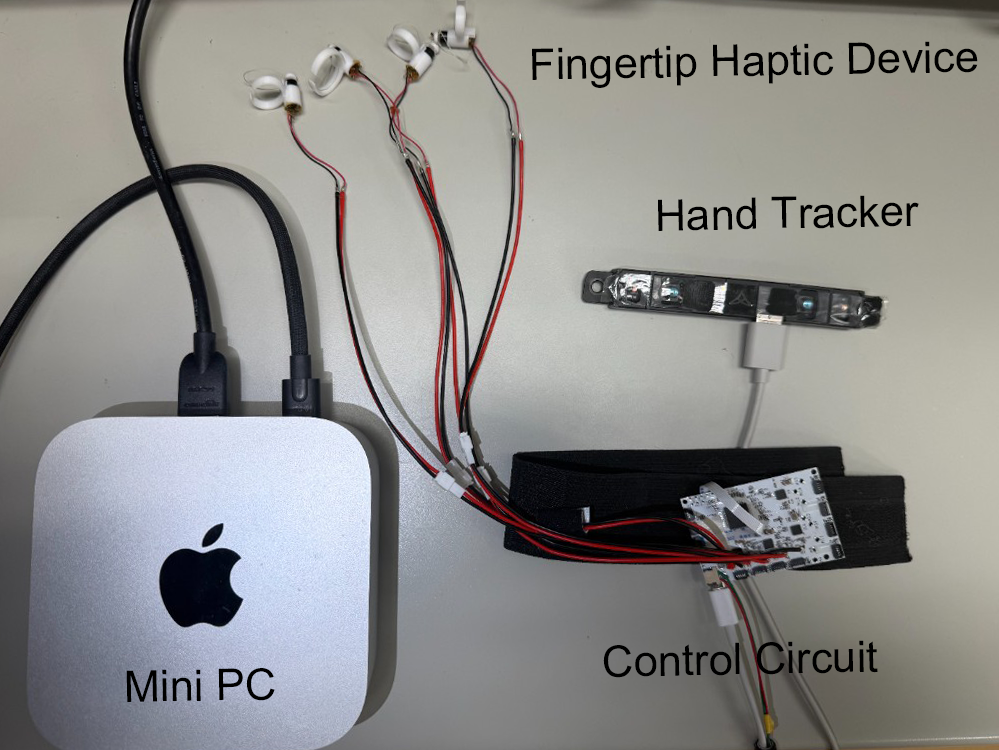
\includegraphics[width=0.85\linewidth]{img/hardware_and_wearable_device.png}}
\caption{Hardware used in the experiment. The right side shows the wrist-mounted fixture and driving circuit, while the top shows the fingertip end-effector. Together with Stereo IR-170 tracking, they provide normal-force cues during palpation.}
\label{fig:hardware}
\end{figure}

\subsection{Liver model and lesion configuration}
Under the default configuration used in the physician experience session, the main system parameters are listed in Table~\ref{tab:model}. These parameters are intended to support stable and perceptible interactive demonstration rather than to claim strict physiological calibration. In this work, the judgment of realism is based on two aspects: first, the relatively credible deformation and volume behavior supported by the underlying technical validation; second, the physician's task performance and subjective feedback during interaction.

\begin{table}[htbp]
\caption{Default Liver Model Parameters}
\label{tab:model}
\begin{tabular}{|l|l|l|}
\hline
Parameter & Value & Description \\
\hline
Base Young's modulus & 7000 Pa & Baseline stiffness of healthy liver tissue \\
Tumor-region Young's modulus & 30000 Pa & Locally increased stiffness in hard regions \\
Poisson ratio & 0.49 & Near-incompressible setting \\
Density & 200 & Empirical parameter used in the current prototype \\
Grouping & 8 $\times$ 6 $\times$ 6 & Local grouped-solving configuration \\
Time step & 0.008 s & Real-time simulation step \\
Volume stabilization & Enabled & Reduces inversion and shrinkage under strong compression \\
\hline
\end{tabular}
\end{table}

To support blind localization experiments, the system predefines three switchable hard-region positions inside the liver. These hard zones are not shown through explicit geometric shape, but are hidden inside the tissue through embedded local stiffness enhancement. This forces participants to infer lesion location only from local deformation and haptic differences, which better matches the essence of palpation. The predefined internal hard-region positions are shown in Fig.~\ref{fig:lesion}, and the interaction interface with multi-finger proxy states is shown in Fig.~\ref{fig:system}. Although the current version already includes basic contact boundaries and global stabilization constraints, it does not yet explicitly model anatomical fixation structures such as the falciform ligament or the triangular ligaments, which was also the most prominent issue raised in expert feedback.

\begin{figure}[htbp]
\centerline{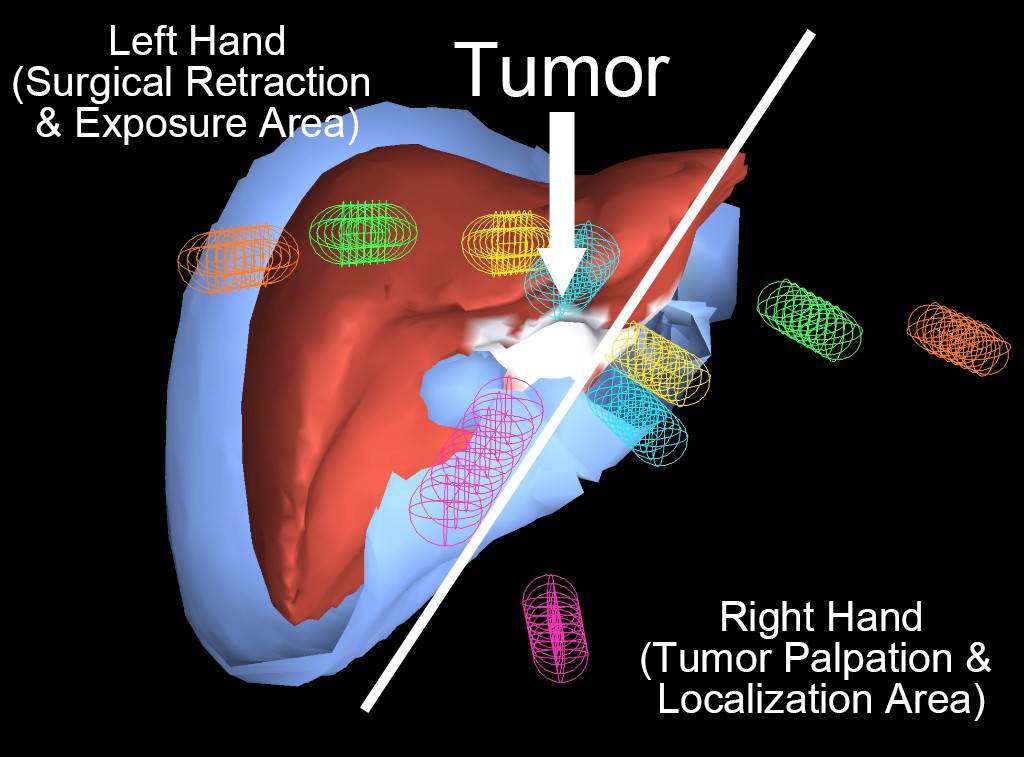
\includegraphics[width=0.9\linewidth]{img/system_simulation_view.png}}
\caption{System interface during runtime. The red mesh denotes the liver surface, the light-blue layer is an auxiliary display, and the colored wireframe bodies are fingertip proxy spheres used for pressing, comparison, and lesion search.}
\label{fig:system}
\end{figure}

\begin{figure}[htbp]
\centerline{\includegraphics[width=0.8\linewidth]{img/lesion_hardzone_points.png}}
\caption{Predefined internal hard-zone positions used in blind localization experiments. The red cube indicates the currently active hard region, which is hidden from the participant during the localization observation sessions.}
\label{fig:lesion}
\end{figure}

\section{Experimental Design and Evaluation Metrics}
\subsection{Application-related validation of the published simulation core}
The core algorithm and most systematic benchmarks of GB-cFEM were already reported in \cite{ref6}. In this paper, we reproduce only the subset of validation results most directly related to deployment in the liver palpation system, mainly to show that the simulation core is suitable as the real-time computational basis of the current system:
\begin{enumerate}
\item Large-deformation accuracy: comparison of displacement response between the proposed method and XPBD under identical material parameters and loading conditions, using VegaFEM as a high-accuracy reference.
\item Near-incompressible volume preservation: under large dragging at different Poisson ratios, the maximum and mean deviations of the volume ratio $V/V_0$ are measured.
\item Directional response validation: force-displacement slopes under loading from different directions are compared to examine whether the system can stably transmit direction-dependent mechanical differences.
\item Real-time performance and scalability: the physics frame rate is measured under different tetrahedral mesh sizes to assess interactivity on standard CPU hardware.
\end{enumerate}

\subsection{Preliminary clinical validation and localization-efficiency evaluation}
One surgeon participated in the system evaluation. The participant profile is listed in Table~\ref{tab:participant}. The goal of this pilot study was to obtain an initial indication of the practical utility of lightweight haptic feedback in a concrete clinical localization task. The evaluation setup is shown in Fig.~\ref{fig:eval}. The participant first watched an approximately five-minute system demonstration, and then completed free exploration, blind lesion localization across a no-haptic session and a haptic-assisted session with different lesion positions, and clinical relevance evaluation.

\begin{table}[htbp]
\caption{Participant Profile}
\label{tab:participant}
\begin{tabular}{|l|l|}
\hline
Attribute & Information \\
\hline
Professional title & Intermediate \\
Clinical experience & 7 years \\
Specialty & Surgery \\
Surgery-related experience & 2 years \\
\hline
\end{tabular}
\end{table}

\begin{figure}[htbp]
\centerline{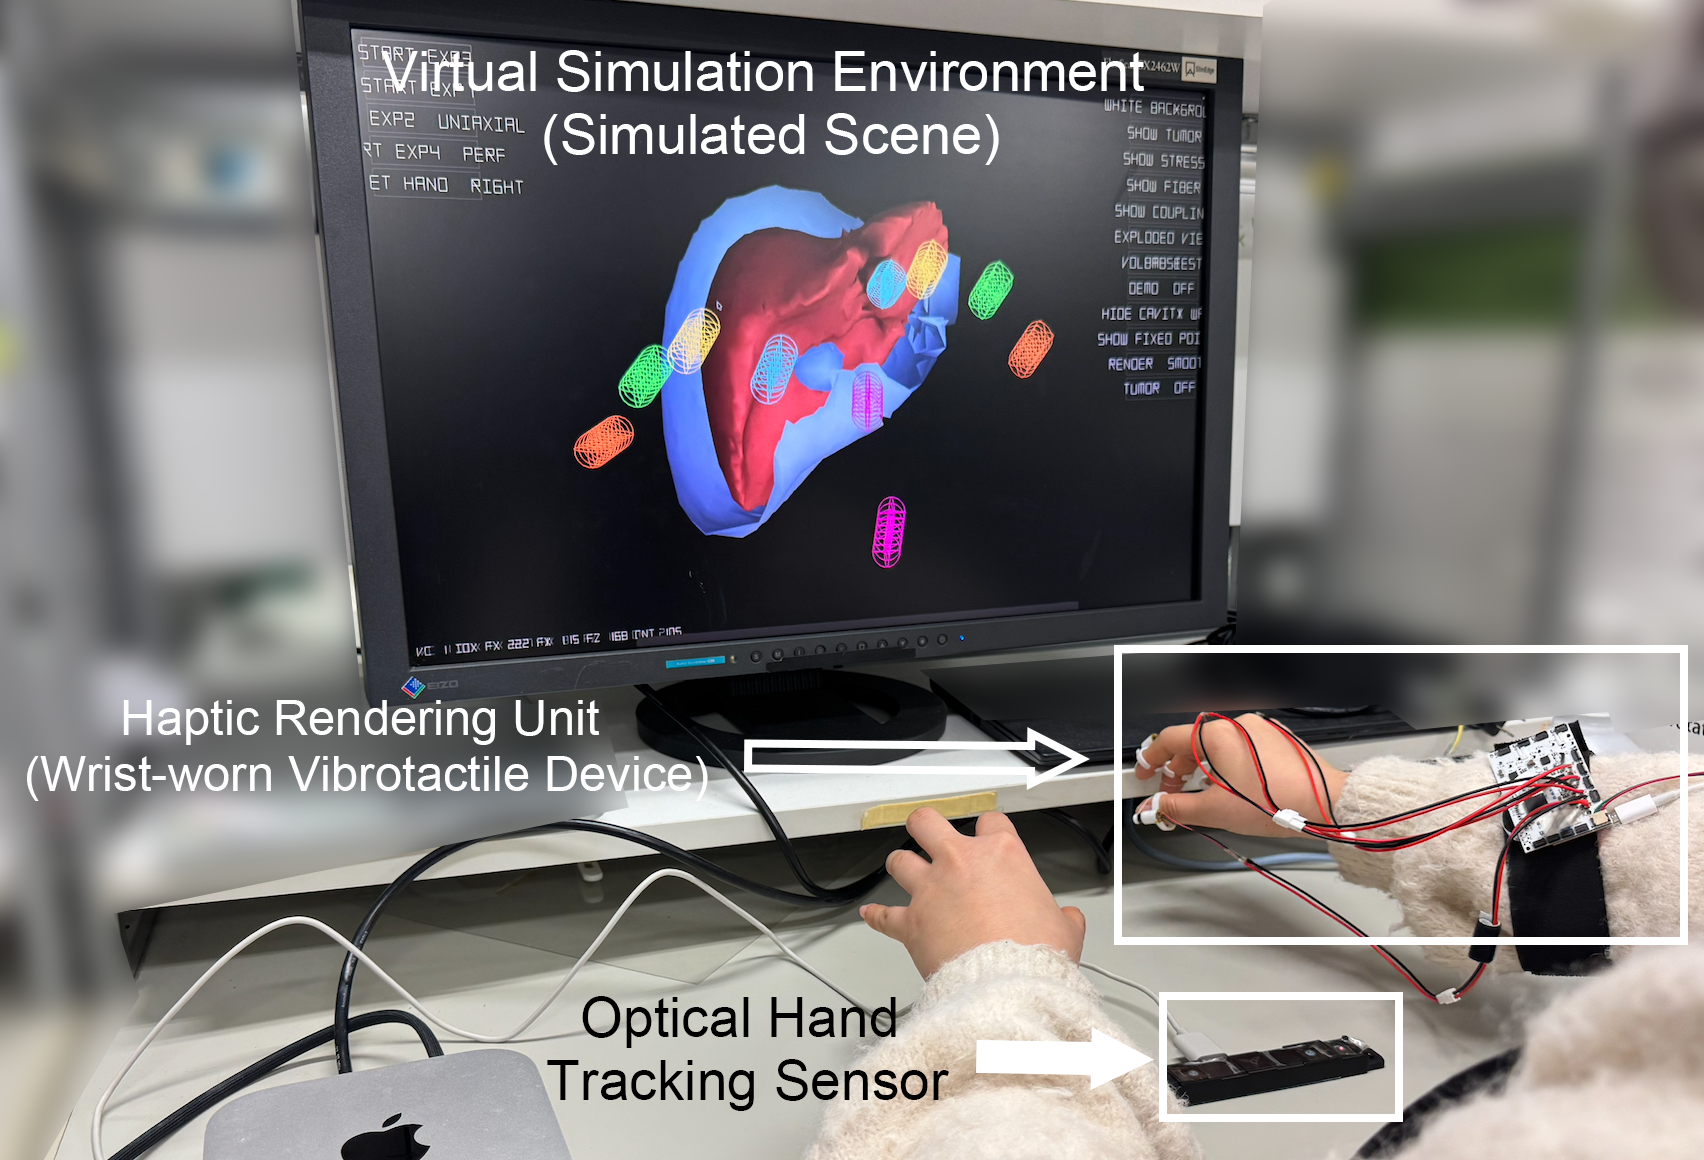
\includegraphics[width=0.85\linewidth]{img/expert_evaluation_setup.png}}
\caption{Expert formative evaluation setup. The participant performs virtual palpation through hand motion while receiving 1-DOF force feedback, and the screen shows real-time liver deformation together with proxy-body positions.}
\label{fig:eval}
\end{figure}

\begin{table}[htbp]
\caption{Evaluation Tasks}
\label{tab:tasks}
\begin{tabular}{|l|l|l|l|}
\hline
Task & Goal & Condition & Recorded content \\
\hline
Task A: Free exploration & Observe interaction fidelity and naturalness & Freely touch the liver and verbalize thoughts & Subjective comments and operation behavior \\
Task B: Blind lesion localization & Observe lesion-search behavior across two sessions & Session 1: no haptics; Session 2: haptic on with changed lesion position & Success, operation strategy, and verbal report \\
Task C: Clinical relevance evaluation & Judge training value and information expressiveness & Press different regions and compare resistance & Semi-structured interview and Likert ratings \\
\hline
\end{tabular}
\end{table}

\subsection{Metrics for formative evaluation}
Following related work on medical simulation, we recorded three classes of metrics. The first class comprises behavioral measures, including whether lesion search succeeded and whether operation strategy changed. The second class comprises subjective evaluation, including spoken feedback during free exploration and structured comments on clinical relevance. The third class comprises scale ratings summarizing educational value, soft-tissue information expression, and realism of force feedback. Because the sample size was one and the lesion conditions were not counterbalanced, no statistical inference was performed; instead, the study emphasizes descriptive results and mechanism-oriented interpretation.

\section{Results}
\subsection{Technical validation results}
\subsubsection{Large-deformation accuracy and real-time performance}
This result reproduces and adapts part of \cite{ref6}. Compared with VegaFEM, the simulation core used in this system exhibits an average displacement error of about 17.9\% under three loading magnitudes, whereas XPBD Fast exceeds 50\%, as shown in Table~\ref{tab:disp} and Fig.~\ref{fig:disp}. More importantly, the proposed core still reaches about 83 FPS at a computational cost of about 12 ms per frame, meeting the real-time requirement of the interactive system. Although XPBD can achieve higher FPS with fewer substeps, its displacement response is too soft, while higher-accuracy settings sacrifice interactivity.

\begin{table}[htbp]
\caption{Large-Deformation Comparison}
\label{tab:disp}
\begin{tabular}{|l|l|l|l|l|}
\hline
Metric & Proposed method & XPBD Fast & XPBD Ref & VegaFEM \\
\hline
Mean displacement error & 17.9\% & 50.8\% & 43.6\% & 0\% (reference) \\
Mean runtime & 12.0 ms & 7.9 ms & 59.2 ms & -- \\
Frame rate & 83.3 FPS & 126.6 FPS & 16.9 FPS & -- \\
\hline
\end{tabular}
\end{table}

\begin{figure}[htbp]
\centerline{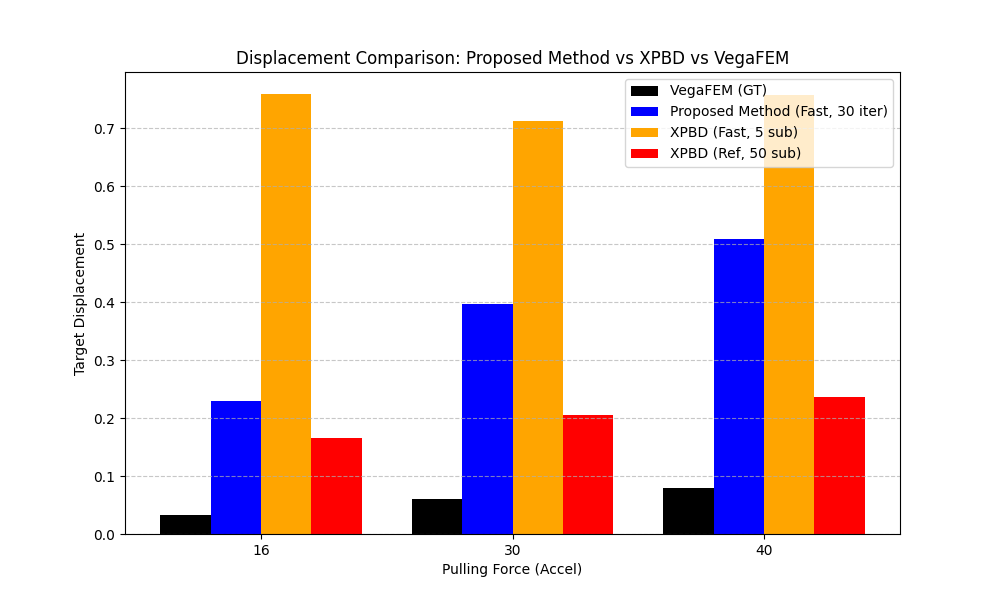
\includegraphics[width=0.9\linewidth]{../out/experiment1/displacement_comparison.png}}
\caption{Comparison of displacement under large deformation.}
\label{fig:disp}
\end{figure}

This result indicates that the simulation core used by the system does not simply trade accuracy for speed, but maintains a more stable stiffness representation than XPBD within an interactive range, which is especially important for lesion palpation.

\subsubsection{Near-incompressible volume preservation}
Part of this result is reproduced from \cite{ref6}. Under near-incompressible settings typical of highly hydrated soft tissues such as the liver, the simulation core used here shows better volume stability than XPBD and remains close to VegaFEM, as shown in Table~\ref{tab:volume} and Fig.~\ref{fig:volume}. In particular, at $\nu = 0.47$, the mean volume deviation is 0.92\% and the maximum deviation is 1.35\%, outperforming XPBD under the same condition.

\begin{table}[htbp]
\caption{Volume Preservation Comparison}
\label{tab:volume}
\begin{tabular}{|l|l|l|l|}
\hline
Method & Poisson ratio & Maximum volume deviation & Mean volume deviation \\
\hline
Proposed method & 0.28 & 1.88\% & 1.31\% \\
Proposed method & 0.47 & 1.35\% & 0.92\% \\
XPBD & 0.28 & 7.27\% & 1.84\% \\
XPBD & 0.47 & 1.59\% & 1.29\% \\
VegaFEM & 0.28 & 1.94\% & 1.28\% \\
VegaFEM & 0.47 & 1.47\% & 0.80\% \\
\hline
\end{tabular}
\end{table}

\begin{figure}[htbp]
\centerline{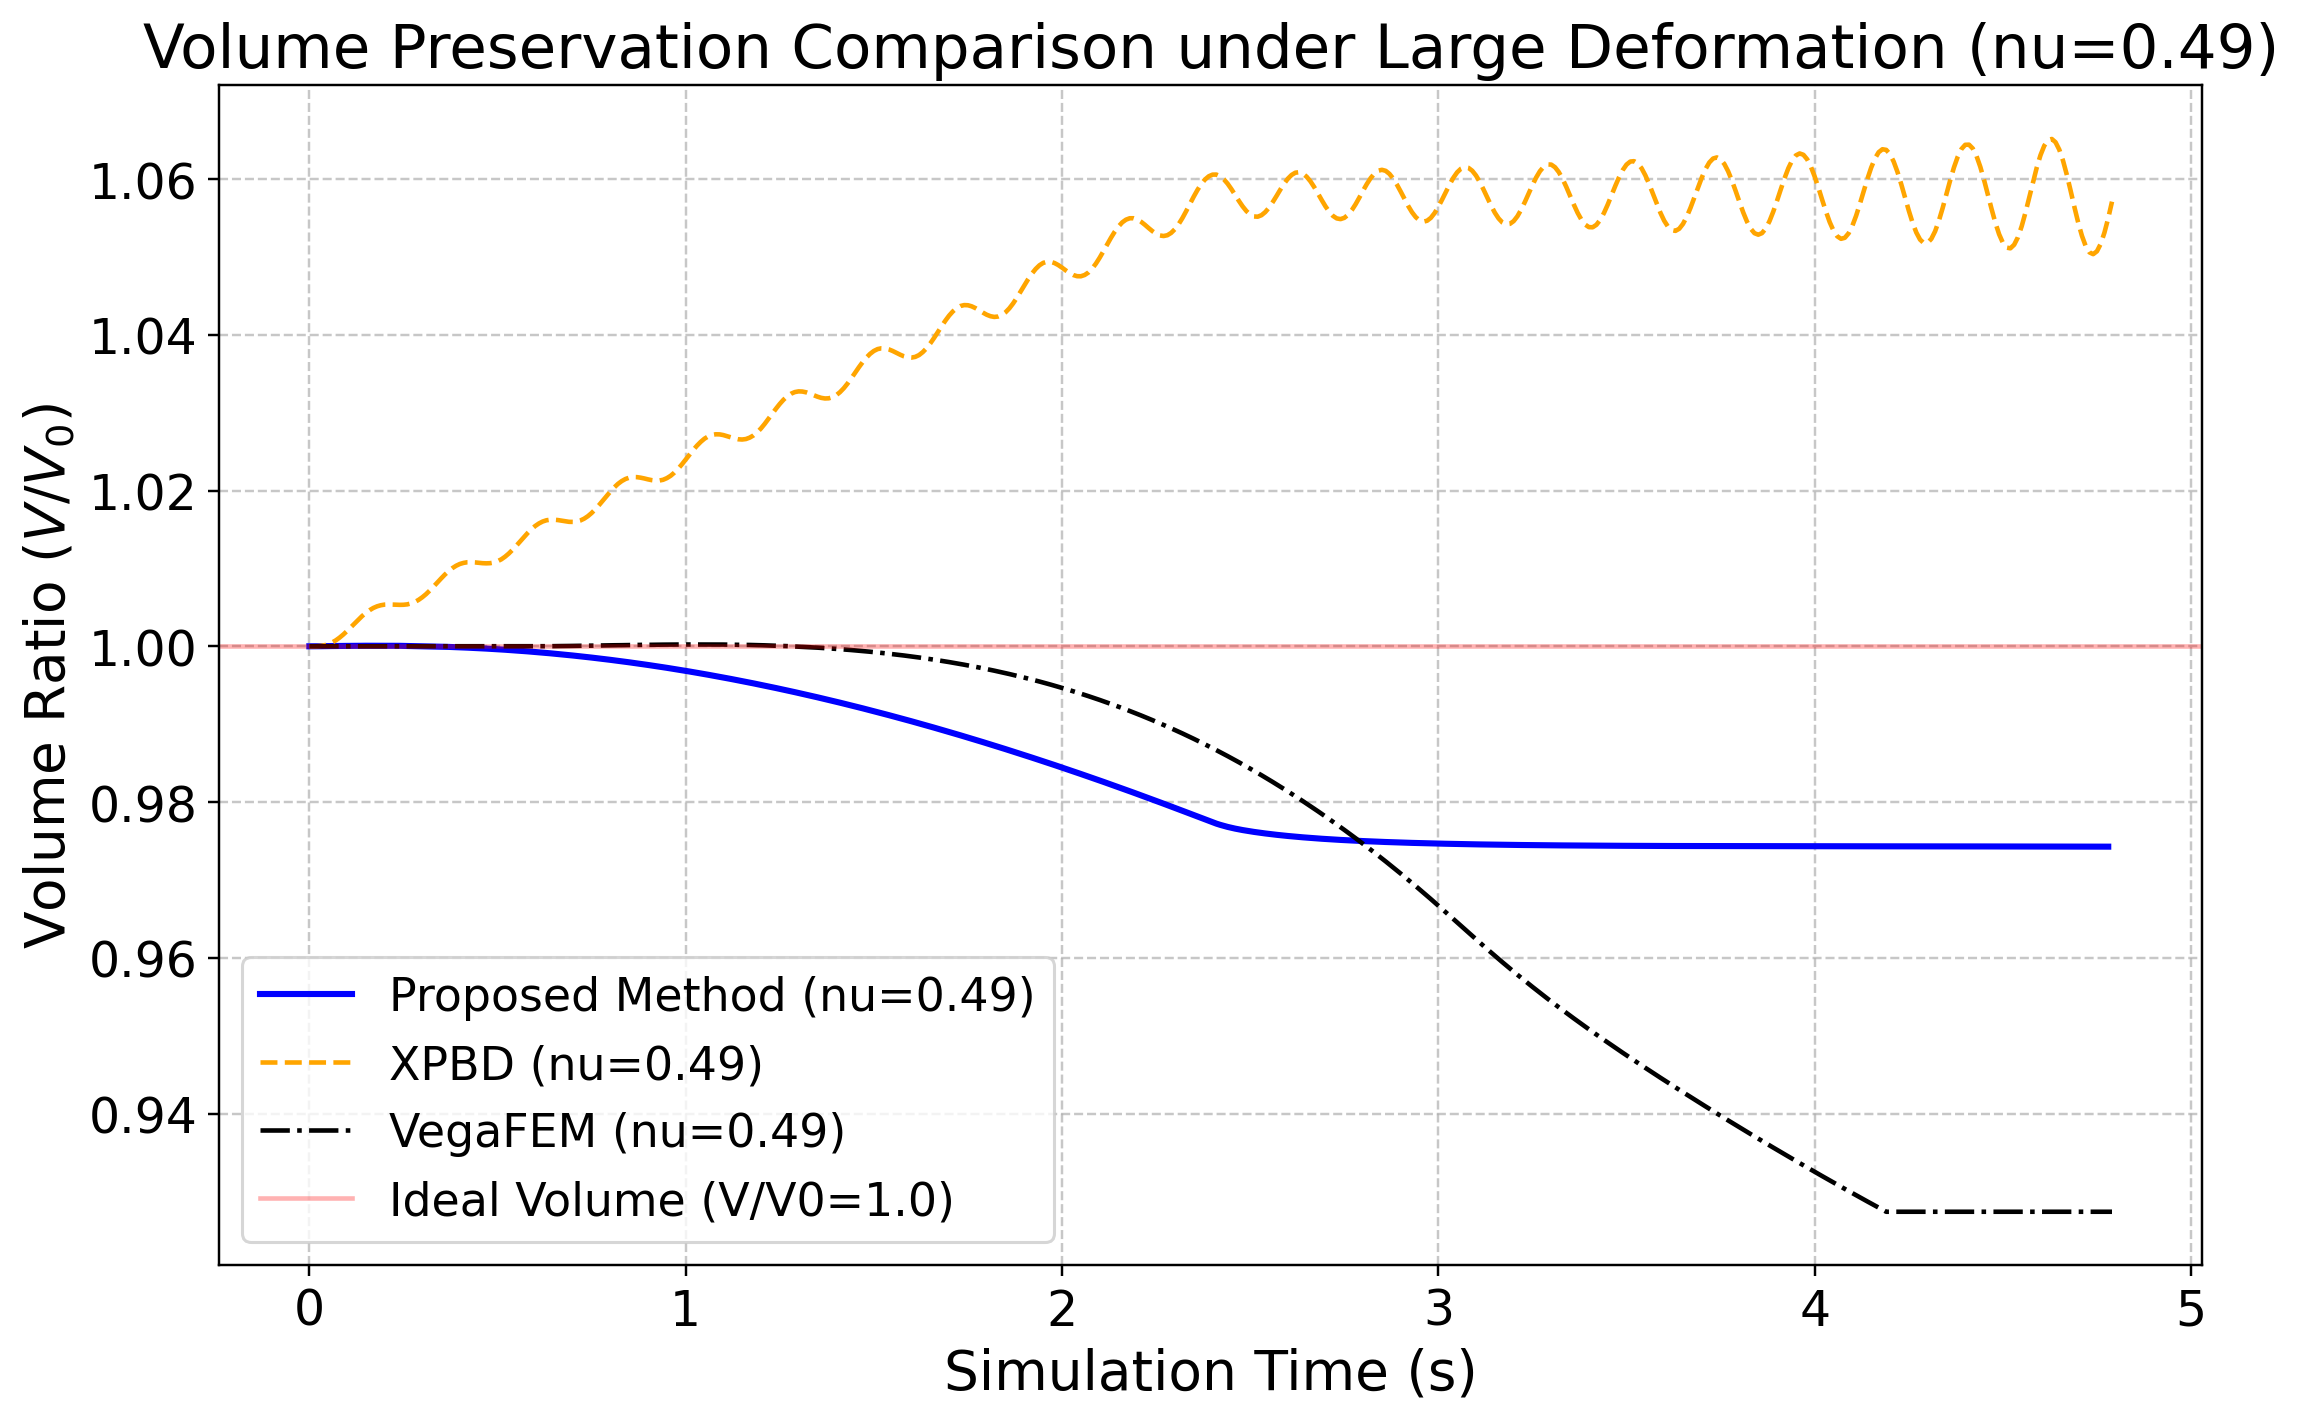
\includegraphics[width=0.9\linewidth]{../out/experiment2/volume_preservation_comparison.png}}
\caption{Comparison of volume preservation.}
\label{fig:volume}
\end{figure}

This suggests that under large pressing and dragging, the proposed method is less likely to produce unrealistic shrinkage or collapse artifacts, thereby providing a more consistent geometric basis for subsequent haptic mapping.

\subsubsection{Directional response}
This validation reproduces the basic setting in \cite{ref6}. The purpose is not to fully reconstruct complex biological fiber mechanics, but to confirm whether the simulation core can support and stably transmit direction-dependent mechanical differences. The result shows that under the current configuration, the apparent stiffness ratio between the X and Y directions is about 2.6, indicating that direction-dependent material settings can be translated into measurable mechanical output.

\begin{table}[htbp]
\caption{Directional Response}
\label{tab:aniso}
\begin{tabular}{|l|l|l|l|}
\hline
Condition & X-axis stiffness (N/m) & Y-axis stiffness (N/m) & Stiffness ratio \\
\hline
Isotropic & 1656.2 & 639.7 & 2.59 \\
Anisotropic & 1687.3 & 649.8 & 2.60 \\
\hline
\end{tabular}
\end{table}

\begin{figure}[htbp]
\centerline{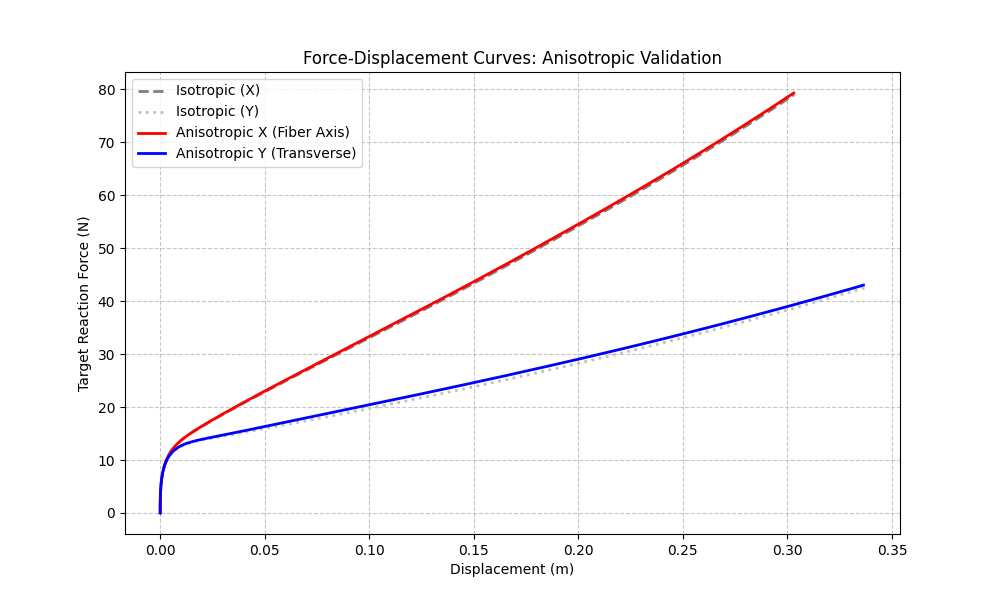
\includegraphics[width=0.9\linewidth]{../out/experiment3/force_displacement_curves.png}}
\caption{Force-displacement curves under directional-response tests.}
\label{fig:aniso}
\end{figure}

\subsubsection{Real-time performance and scalability}
Following the performance framework in \cite{ref6}, we reevaluated runtime behavior under different mesh sizes. As shown in Table~\ref{tab:fps} and Fig.~\ref{fig:fps}, the simulation core reaches 219.24 FPS at about 7,790 tetrahedra and still maintains about 20.2 FPS at about 35,486 tetrahedra. By comparison, VegaFEM reaches only 5.52 FPS at about 18,245 tetrahedra, while the high-accuracy XPBD reference reaches 16.27 FPS at about 20,061 tetrahedra.

\begin{table}[htbp]
\caption{Runtime and Scalability}
\label{tab:fps}
\begin{tabular}{|l|l|l|l|}
\hline
Method & Mesh size & FPS & Note \\
\hline
Proposed method & 7,790 tets & 219.24 & Clearly above real-time needs \\
Proposed method & 35,486 tets & 20.2 & Maintains basic interactivity \\
XPBD Ref & 20,061 tets & 16.27 & High-accuracy configuration is costly \\
VegaFEM & 18,245 tets & 5.52 & Difficult to interact with in real time \\
\hline
\end{tabular}
\end{table}

\begin{figure}[htbp]
\centerline{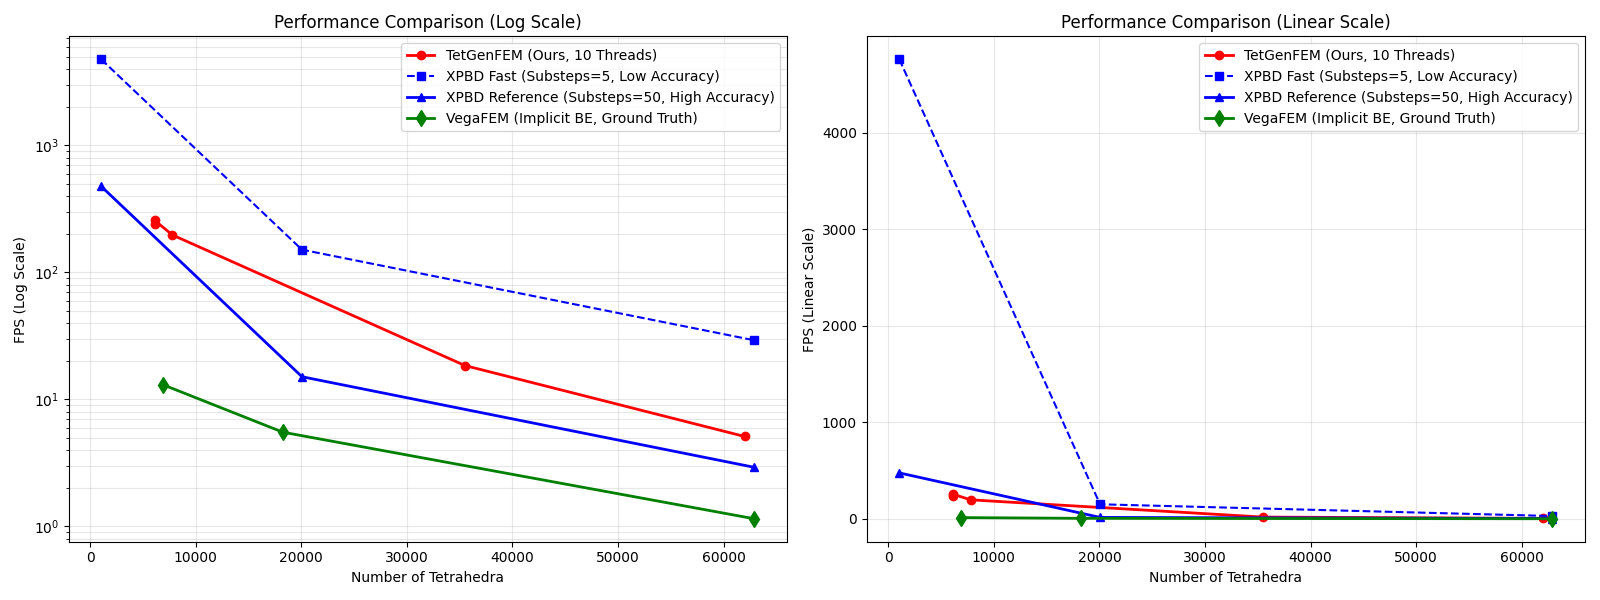
\includegraphics[width=0.9\linewidth]{../out/experiment4/comparison_fps.png}}
\caption{Overall runtime trend across methods and mesh scales.}
\label{fig:fps}
\end{figure}

Although the mesh sizes used by different methods are not exactly matched point by point, the result is sufficient to indicate that the GB-cFEM route used in this system can support medical demonstration and interactive tasks on a consumer-grade CPU without relying on heavier high-end computing resources.

\subsection{Preliminary clinical validation results}
\subsubsection{Interaction fidelity during free exploration}
In the free-touch task, the participant first performed multi-finger pressing on different parts of the liver surface, then attempted to lift the thin edge of the liver, and explored dynamic changes in force feedback by varying indentation depth. Together with comparative palpation between the preset lesion region and healthy tissue, the participant evaluated the system from both anatomical and physical perspectives.

First, the participant pointed out distortion in material modulus. The current liver soft-tissue model was described as overly elastic, with a sensation closer to homogeneous soft gel than to fibrous biological tissue. A real liver exhibits nonlinear stiffness and is wrapped by Glisson's capsule, which yields an ``initial resistance, then constrained compression'' characteristic. In contrast, the current model deforms too easily under pressure.

Second, anatomical constraints are missing. The system lacks mechanical modeling of supporting ligaments such as the falciform ligament and the left and right triangular ligaments. The participant observed that when the liver was pushed from the side, the model behaved like a floating object undergoing global translation rather than ligament-limited rotation or local deformation. This anatomical simplification disconnects the feedback logic from real clinical manipulation.

Third, the participant noted a deviation in interaction paradigm. Bare-hand palpation is relevant in clinical diagnosis, but in surgical scenarios the main interaction medium is the surgical instrument. Direct hand-tracking interaction reduces the learning barrier, but at the cost of task validity for surgical simulation, making the experience closer to physical examination than intraoperative manipulation.

These comments define the current usage scope of the system as a task-focused prototype for expressing lesion-related tactile cues, and they clarify which mechanical and boundary conditions still need to be added to approach clinical-grade surgical simulation.

\subsubsection{Behavioral observation during lesion localization sessions}
Task B was interpreted as a descriptive observation rather than a controlled comparison. In the no-haptic session, the participant relied mainly on visual deformation. Behavioral observation showed that the initial strategy involved small surface indentations, but after failing to obtain useful stiffness cues, the participant gradually shifted to broad, irregular pulling and heavy squeezing over a wider area.

After haptic feedback was introduced in a later session with a different hidden-lesion position, the participant's strategy changed to local comparative palpation. During this session, the participant verbally reported perceiving differences in resistance and used those differences to narrow the search to an approximate lesion region. This behavioral change is consistent with the intended role of the 1-DOF cue, namely to provide a usable local stiffness contrast even when the lesion is not visually identifiable.

Because this formative observation involved only one participant and a non-balanced sequence with different lesion positions, it should not be interpreted as causal proof that haptic feedback improved localization performance. Instead, the result is retained here only as preliminary descriptive evidence of system usability and task-related behavior.

\subsubsection{Clinical relevance and force-rendering quality evaluation}
In Task C, the participant actively performed continuous sliding exploration and deep pressing over the liver surface while cross-checking fingertip force sensation against the on-screen deformation. Based on these dynamic palpation behaviors, the participant proposed several directions for improvement from a perceptual and psychophysical perspective.

The first issue is the lack of directional richness. The current feedback reflects only one-dimensional normal resistance and lacks tangential force and more complex reaction-force distribution. This unidimensional haptic rendering cannot reproduce the sense of tissue enclosure that occurs when a real fingertip is pressed into soft tissue and compressed by the surrounding material.

The second issue concerns haptic refresh rate and continuity. The participant subjectively perceived an intermittent or step-like sensation, indicating a synchronization problem between the haptic update loop and the physics simulation engine. Discontinuous feedback makes it harder to form a stable spatial haptic map and reduces the ability to finely distinguish tissue characteristics, such as cystic versus solid nodules.

\begin{table}[htbp]
\caption{Likert-Scale Evaluation}
\label{tab:likert}
\begin{tabular}{|l|l|l|}
\hline
Evaluation dimension & Score (out of 5) & Interpretation \\
\hline
Educational value & 4/5 & The participant considered the ``soft tissue + haptics'' direction meaningful for training \\
Soft-tissue information expression & 4/5 & The system provided richer lesion cues than vision alone \\
Force-feedback realism & 3/5 & Helpful, but still simplified due to limited dimensionality and continuity \\
\hline
\end{tabular}
\end{table}

These ratings show that the participant recognized both the educational value and the soft-tissue information content of the system, while judging the realism of force feedback as moderate. In other words, the prototype can already convey useful information, but it has not yet reached the level of high-fidelity clinical haptic reconstruction. This conclusion is consistent with the engineering scope of the present work.

\section{Discussion}
\subsection{From algorithm validation to system-prototype evaluation}
The main concern of this paper is not to repeat the claim that one solver outperforms another on a benchmark, but to ask whether a physics core with basic credibility, namely the one reported in \cite{ref6}, can truly support a palpation interaction system that physicians can use and evaluate. The partially reproduced technical validation reaffirms that the simulation core can support real-time large deformation in the intended application setting, while the expert evaluation provides an initial descriptive observation of how lesion-search behavior changes after haptic cues are introduced. This transition from algorithm benchmarking to system-prototype evaluation matches the application-oriented goal of the paper.

\subsection{Application focus and future evolution of the system}
For the core task of liver lesion localization, the current system successfully expresses useful lesion-related features through normal-force-based stiffness feedback. To further improve overall surgical simulation fidelity, future work can evolve along several directions. First, more complex material models can be introduced to capture capsule effects and nonlinear compression behavior. Second, ligament and abdominal support constraints can be added to improve the organ's sense of anchoring. Third, the interaction paradigm can be extended from direct palpation toward instrument-mediated manipulation. Fourth, while preserving the lightweight advantage of the 1-DOF solution, the feedback controller can be further refined with tangential compensation and improved continuity.

\subsection{Next research directions}
The next stage of work will prioritize the following directions. First, motivated by the descriptive localization observation reported here, we plan to conduct a larger clinical evaluation involving multiple surgeons and a properly counterbalanced protocol to obtain statistically meaningful user feedback. Second, we will add more complete ligament and abdominal boundary modeling to improve macroscopic support behavior of the organ. Finally, we will explore surgical-tool proxy interaction so that the current palpation training platform can be extended toward a more complete minimally invasive operation training scenario.

\section{Conclusion}
This paper investigated the system-level coupling among real-time soft-tissue simulation, bimanual interaction, 1-DOF normal-force mapping, and formative evaluation through the development of a real-time liver palpation system. In contrast to \cite{ref6}, which focused on algorithmic derivation, the present study emphasizes how a previously published physics simulation core can be organized into a runnable and evaluable palpation prototype.

Application-oriented technical validation supports the suitability of the simulation core for large deformation and real-time interaction. Through formative evaluation with a single expert participant, we further observed that even with a 1-DOF haptic device, targeted normal-force feedback may encourage a shift toward local comparative palpation and may help the operator perceive local resistance differences. This work represents an initial feasibility study of a system prototype. Because the clinical observation was single-case and non-counterbalanced, it is intended only as descriptive evidence rather than as proof of haptic efficacy. The physician's feedback nevertheless clearly indicates directions for future improvement and evolution.

Overall, this paper presents a lightweight engineering route that integrates a published GB-cFEM core, Ultraleap Stereo IR-170 bimanual tracking, and 1-DOF haptic output. At relatively low hardware cost, the prototype achieves a preliminary expression of the force cues required for lesion localization, providing a useful system basis for future large-sample clinical evaluation and for the development of portable medical training platforms.

\begin{thebibliography}{00}
\bibitem{ref1} E. M. Overtoom, M. Horeman, F. Dankelman, J. P. W. Ruurda, and J. J. van den Dobbelsteen, ``Haptic feedback, force feedback, and force-sensing in simulation training for laparoscopy: A systematic overview,'' \emph{J. Surg. Educ.}, 2018, doi:10.1016/j.jsurg.2018.06.008.
\bibitem{ref2} K. Rangarajan \emph{et al.}, ``Systematic review of virtual haptics in surgical simulation: A valid educational tool?,'' \emph{J. Surg. Educ.}, 2020, doi:10.1016/j.jsurg.2019.09.006.
\bibitem{ref3} D. Escobar-Castillejos, J. Noguez, L. Neri, A. Magana, and B. Benes, ``A review of simulators with haptic devices for medical training,'' \emph{J. Med. Syst.}, 2016, doi:10.1007/s10916-016-0459-8.
\bibitem{ref4} E. W. Riddle, D. Kewalramani, M. Narayan, and D. B. Jones, ``Surgical simulation: Virtual reality to artificial intelligence,'' \emph{Curr. Probl. Surg.}, 2024, doi:10.1016/j.cpsurg.2024.101625.
\bibitem{ref5} H. P. Bui, S. Tomar, and S. P. A. Bordas, ``Corotational cut finite element method for real-time surgical simulation: Application to needle insertion simulation,'' \emph{Comput. Methods Appl. Mech. Eng.}, 2019, doi:10.1016/j.cma.2018.10.023.
\bibitem{ref6} S. Wang, Y. Xu, and S. Hasegawa, ``Group-based corotational FEM for real-time large deformation simulation,'' \emph{IEEE Access}, 2025, doi:10.1109/ACCESS.2025.3616629.
\bibitem{ref7} S. Bouaziz, S. Martin, T. Liu, L. Kavan, and M. Pauly, ``Projective dynamics: Fusing constraint projections for fast simulation,'' \emph{ACM Trans. Graph.}, 2014, doi:10.1145/2601097.2601116.
\bibitem{ref8} T. Liu, S. Bouaziz, and L. Kavan, ``Towards real-time simulation of hyperelastic materials,'' arXiv:1604.07378, 2016.
\bibitem{ref9} J. Bender, M. Muller, M. A. Otaduy, M. Teschner, and M. Macklin, ``A survey on position-based simulation methods in computer graphics,'' \emph{Comput. Graph. Forum}, 2014, doi:10.1111/cgf.12346.
\bibitem{ref10} M. Muller, B. Heidelberger, M. Hennix, and J. Ratcliff, ``Position based dynamics,'' \emph{J. Vis. Commun. Image Represent.}, 2007, doi:10.1016/j.jvcir.2007.01.005.
\bibitem{ref11} M. Macklin, M. Muller, and N. Chentanez, ``XPBD: Position-based simulation of compliant constrained dynamics,'' in \emph{Proc. Motion in Games}, 2016, doi:10.1145/2994258.2994272.
\bibitem{ref12} H. Wu \emph{et al.}, ``Interactive hepatic parenchymal transection simulation with haptic feedback,'' \emph{Virtual Reality Intell. Hardware}, 2021, doi:10.1016/j.vrih.2021.09.003.
\bibitem{ref13} F. G. Hamza-Lup, C. M. Bogdan, and A. Seitan, ``Haptic simulator for liver diagnostics through palpation,'' in \emph{Med. Meets Virtual Reality 19}, 2012, doi:10.3233/978-1-61499-022-2-156.
\bibitem{ref14} W. Agboh, O. Yalcin, and V. Patoglu, ``A six degrees of freedom haptic interface for laparoscopic training,'' in \emph{IEEE/RSJ IROS}, 2016, doi:10.1109/IROS.2016.7759187.
\bibitem{ref15} O. Bjelland \emph{et al.}, ``Haptic rendering using reality-based force profiles in surgical simulation,'' \emph{IEEE Trans. Haptics}, 2025, doi:10.1109/TOH.2025.3570810.
\bibitem{ref16} L. He \emph{et al.}, ``Energy-based haptic rendering for real-time surgical simulation,'' \emph{Comput. Graphics}, 2026, doi:10.1016/j.cag.2025.104524.
\bibitem{ref17} W. Hou, P. X. Liu, and M. Zheng, ``A new model of soft tissue with constraints for interactive surgical simulation,'' \emph{Comput. Methods Programs Biomed.}, 2019, doi:10.1016/j.cmpb.2019.03.018.
\end{thebibliography}

\EOD

\end{document}
